\chapter{Deep Learning}

\section{Machine learning}

\begin{figure}[H]
    \centering
    \begin{minipage}{0.48\textwidth}
        \centering
        \begin{tikzpicture}

            \node [rectangle, draw=black!60, fill=light_blue, very thick, minimum height=3em] (mid) at (0,0) {\textbf{Computer}};
            \node (l1) at (-3,0.3) {Input};
            \node (l2) at (-3,-0.3) {Program};
            \node (r)  at (3,0) {Output};
        
            \draw [very thick, draw = black,->] (mid)--(r);
            \draw [very thick, draw = black,->] (l1.east)--(-1.1,0.3);
            \draw [very thick, draw = black,->] (l2.east)--(-1.1,-0.3);
        
        \end{tikzpicture}
        \caption{Traditional Programming}
    \end{minipage}
    \begin{minipage}{0.48\textwidth}
        \centering
        \begin{tikzpicture}

            \node [rectangle, draw=black!60, fill=light_blue, very thick, minimum height=3em] (mid) at (0,0) {\textbf{Computer}};
            \node (l1) at (-3,0.3) {Input};
            \node (l2) at (-3,-0.3) {Output};
            \node (r)  at (3,0) {Program};
        
            \draw [very thick, draw = black,->] (mid)--(r);
            \draw [very thick, draw = black,->] (l1.east)--(-1.1,0.3);
            \draw [very thick, draw = black,->] (l2.east)--(-1.1,-0.3);
        
        \end{tikzpicture}
        \caption{Machine Learning}
    \end{minipage}
\end{figure}

\subsection{Important concepts}

\subsubsection{Model}

A mathematical description that explains the relation between input x and output y. (输入输出的映射关系)

Defined as a function $y=f_W(x)$ with parameters dentoed by W. 

\begin{wrapfigure}{r}{0.38\textwidth}
    \centering
    \begin{tikzpicture}
        \node [rectangle, draw=black] (mid)  {$f_W$};
        \node (a) [left=3em of mid] {Input x};
        \node (b) [right=3em of mid] {Output y};

        \draw[very thick, draw = black, ->] (a)--(mid);
        \draw[very thick, draw = black, ->] (mid)--(b);
    \end{tikzpicture}
    \caption{Model}
\end{wrapfigure}

Problem types: 
\begin{itemize}
    \item Regression(回归): y is a real number.
    \item Classification(分类): y is a discrete label. 
\end{itemize}

\subsubsection{Supervised learning(监督学习)}

Find $f_W$ from labeled data. 

labeled data: exisiting (x,y) pairs, called training data.

\begin{wrapfigure}{r}{0.38\textwidth}
    \centering
    \begin{tikzpicture}
        \node [rectangle, draw=black] (mid)  {$f_W$};
        \node (a) [left=3em of mid] {Input x};
        \node (b) [right=3em of mid] {Output y};
        \node [rectangle, draw=black] (c) [above=2em of mid] {Training algorithm};
        \node [rectangle, draw=black, text width=10em,text centered,] (d) [above=2em of c] {Labeled data};

        \draw[very thick, draw = black, ->] (a)--(mid);
        \draw[very thick, draw = black, ->] (mid)--(b);
        \draw[very thick, draw = black, ->] (c)--(mid);
        \draw[very thick, draw = black, ->] (d)--(c);
    \end{tikzpicture}
    \caption{Supervised learning}
\end{wrapfigure}

Tow phases:
\begin{enumerate}
    \item Training: given labeled data, find $f_W$. (model fitting, 模型拟合)
    \item Testing: given $f_W$ and a new x, find y. (inference, 模型推理)
\end{enumerate}

\subsubsection{General pipeline}
\begin{enumerate}
    \item Define the problem: What is x and y. 
    \item Collect training data: (x,y) pairs.
    \item Design a model: What is the form of $f_W$.
    \item Model training
    \begin{enumerate}
        \item Define a loss function $l(W)$.
        \item Find optimal W that minimizes $l(W)$ using some optimzation algorithm. 
    \end{enumerate}
    \item Testing(application): Given a new data x, predict y with the learning $f_W$. 
\end{enumerate}

Example: 
\begin{itemize}
    \item 回归: 最小二乘
    \item 分类: 图像分类
\end{itemize}
\section{Linear classifier(线性分类器)}
\subsection{Classification model}
\begin{itemize}
    \item Input x: image
    \item Output y: class scores
\end{itemize}

\begin{figure}[H]
    \centering
    \begin{tikzpicture}
        \node [text centered, text width=12em] (pic) at (-4.5,0) {picture: $[32\times 32\times 3]$ \\ array of numbers $0\dots 1$\\(3072 numbers total)};
        \node [text width=12em] (output) at (4.5,0) {10 numbers indicating class scoers};
        \node (f) at (0,0.4) {\fcolorbox{light_green}{white}{$f(x,W)$}=\fcolorbox{light_red}{white}{$W$}\fcolorbox{light_blue}{white}{$x$}\fcolorbox{purple}{white}{$+b$}};
        \node [color=light_green] at (-1,1) {$10\times 1$};
        \node [color=light_blue, text centered, text width=5em] at (1,1.3) {image\\$3072\times 1$};
        \node (W) [color=light_red, text centered, text width=14em] at (0.4,-1.3) {$10\times 3072$\\ parameters or ``weight''(权重)};
        \node (b) [text centered, text width=8em, color=purple] at (4,1.5) {bias vector(偏置)\\ $10\times 1$};

        \draw[very thick, draw = black, ->] (pic)--(output);
        \draw[thick, draw = black,color=light_red, ->] (0.4,0.2)--(W);
        \draw[thick, draw = black,color=purple, ->] (f.north east)--(b.south west);
    \end{tikzpicture}
    \caption{Linear classifier}
\end{figure}

\begin{figure}[H]
    \centering
    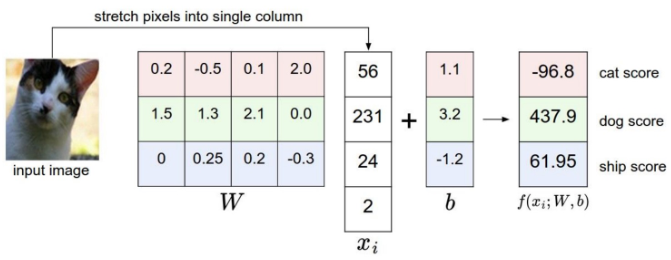
\includegraphics[width=0.68\textwidth]{Lec9/Linear classifier}
    \caption{Example with an image with 4 pixels and 3 classes}
\end{figure}

\subsection{Interpret linear classifier}
When is the score $w^T x+b$ large? 
\begin{itemize}
    \item When $x$ (image) is similar to $w$ (weights). ($w$与$x$越像分数越大)
    \item $w$ represents how an object should look like. ($w$是$W$中一类所对应的一行)
\end{itemize}

We can decide the class label by thresholding the score, then $w^Tx+b=0$ is called decision boundary. 

\begin{figure}[H]
    \centering
    \begin{subfigure}{0.38\textwidth}
        \centering
        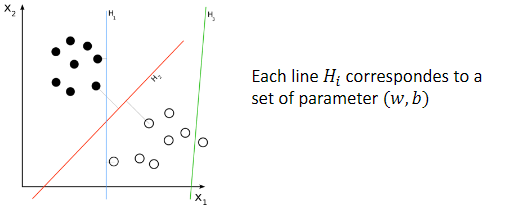
\includegraphics[width=\textwidth]{Lec9/2D}
        \caption{2-class}
    \end{subfigure}
    \begin{subfigure}{0.28\textwidth}
        \centering
        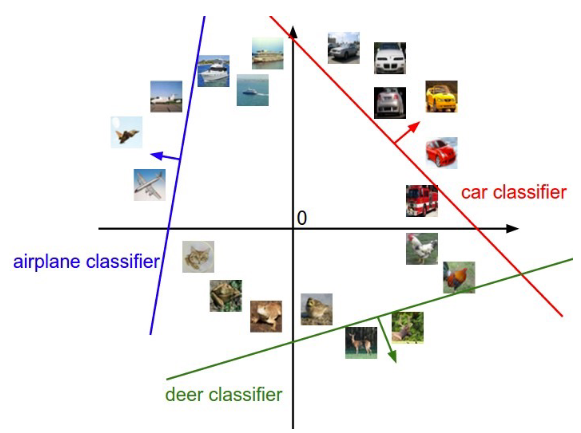
\includegraphics[width=\textwidth]{Lec9/Multi-class}
        \caption{Multi-class}
    \end{subfigure}
    \caption{Linear classifier in 2D}
\end{figure}

若是在2D中, 相近的点表示一个类别, 分类器的作用就是将这些类别划分, 高维情况同理. 

\subsection{Training: find good parameters}
\begin{enumerate}
    \item Difficult to handcraft $w$.
    \item Define a loss (objective) function that quantifies the “goodness” (likelihood) of $w$.
    \item Solve the optimization problem.
\end{enumerate}

\subsection{Loss function of classification}
对分类不能使用MSE loss, 因为labels是离散的而分数是连续的. 

To define a loss function, class labels can be viewed as probabilities. (将离散类别转化为概率)

\begin{enumerate}
    \item Convert scores to probabilities
    \item Compute cross entropy between predicted and true probabilities
\end{enumerate}

\subsubsection{Convert scores to probabilities}

\begin{align*}
    \text{Softmax operator: }\, \sigma (z)_j=\frac{e^{z_j}}{\sum_{k=1}^K e^{z_k}} \, \text{for}\,j=1,\dots,K
\end{align*}

\begin{wrapfigure}{r}{0.38\textwidth}
    \centering
    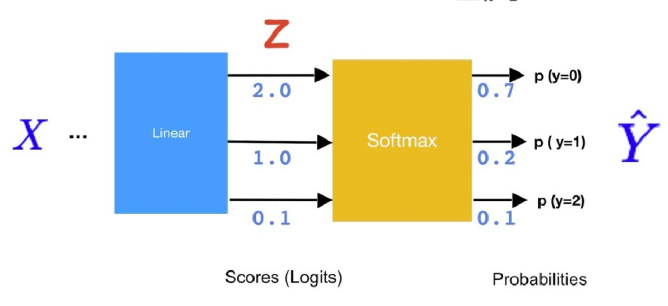
\includegraphics[width=0.3\textwidth]{Lec9/Convert scores to probabilities}
    \caption{Convert scores to probabilities}
\end{wrapfigure}

$z_i$带代表的是类别的分数. 

% \begin{figure}[H]
%     \centering
%     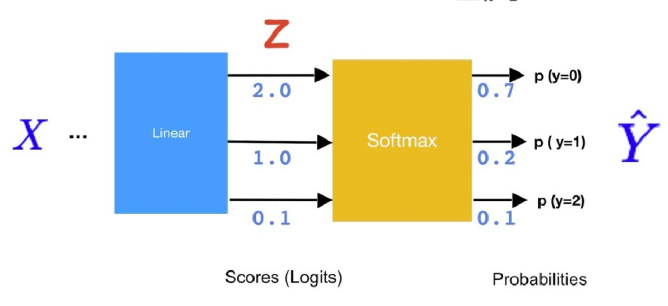
\includegraphics[width=0.38\textwidth]{Lec9/Convert scores to probabilities}
%     \caption{Convert scores to probabilities}
% \end{figure}

\subsubsection{Cross entropy(交叉熵) as loss function}
cross entropy, 在统计上用于衡量分布的距离. 熵越小, 分布越一致. 

分布S, L的交叉熵D(S,L)为
\begin{align*}
    D(S,L)=-\sum_i L_i \log S_i
\end{align*}

\section{Neural networks}

\subsection{Graphical representation}
Perceptron(感知机, 最简单的网络, 为线性分类器)
\begin{figure}[H]
    \centering
    \begin{tikzpicture}
        \node (f) [circle, fill=light_red, draw=black] at (0,4){$f(x)$};
        \node (x1) [circle, fill=light_blue, draw=black] at (-3,0){$x_1$}; 
        \node (x2) [circle, fill=light_blue, draw=black] at (-2,0){$x_2$}; 
        \node (x3) [circle, fill=light_blue, draw=black] at (-1,0){$x_3$}; 
        \node (x4) [circle, fill=light_blue, draw=black] at (0,0){$x_4$}; 
        \node (x5) [circle, fill=light_blue, draw=black] at (1,0){$x_5$}; 
        \node (x6) [circle, fill=light_blue, draw=black] at (2,0){$x_6$}; 
        \node (x7) [circle, fill=light_blue, draw=black] at (3,0){$x_7$};

        \node at (-2.1,1.5) {$w_1$};
        \node at (-1.4,1.5) {$w_2$};
        \node at (-0.7,1.5) {$w_3$};
        \node at (0,1.5) {$w_4$};
        \node at (0.7,1.5) {$w_5$};
        \node at (1.4,1.5) {$w_6$};
        \node at (2.1,1.5) {$w_7$};
        
        \foreach \n in {x1,x2,x3,x4,x5,x6,x7}{\draw[thick, color=light_red, ->] (\n)--(f);}
    \end{tikzpicture}
    \caption{Perceptron}
\end{figure}

\subsection{Limitation of linear model}
However, the data may be NOT linear separable. 

\begin{figure}[H]
    \centering
    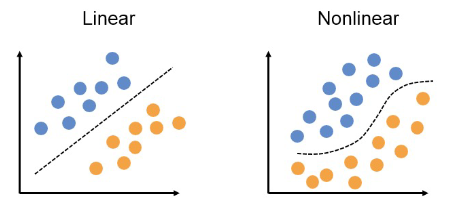
\includegraphics[width=0.68\textwidth]{Lec9/Limitation of linear model}
    \caption{Limitation of linear model}
\end{figure}

\subsection{Activation functions(激活函数)}
To model nonlinearity, add a nonlinear transform, named activation functions. 

\begin{align*}
    f(x)=\sigma(w^T x+b)
\end{align*}

Examples: 
\begin{itemize}
    \item Rectified Linear Unit (ReLU): $\sigma(z)=\max(0,z)$ (\textbf{Electrical pulse} cannot be negative)
    \item Sigmoid:$\sigma(z)=\frac{1}{1+e^{-z}}$ (Map values to probability)
\end{itemize}

\begin{figure}[H]
    \centering
    \begin{minipage}{0.48\textwidth}
        \centering
        \begin{tikzpicture}
            \draw [thick,->] (-2,0)--(2,0);
            \draw [thick,->] (0,0)--(0,3);
            
            \draw [ultra thick, color=light_blue] (-2,0)--(0,0);
            \draw [ultra thick, color=light_blue] (0,0)--(1.5,3);
        \end{tikzpicture}
        \caption{ReLU}
    \end{minipage}
    \begin{minipage}{0.48\textwidth}
        \centering
        \begin{tikzpicture}[yscale=3, xscale=0.4]
            \draw [thick,->] (-5,0)--(5,0);
            \draw [thick,->] (0,0)--(0,1);
            \draw [ultra thick, color=light_blue, domain=-5:5] plot (\x, {1/(1+exp(-\x))});
        \end{tikzpicture}
        \caption{Sigmoid}
    \end{minipage}
\end{figure}

\subsection{Multiple outputs}
To represent multiple outputs.
\begin{figure}[H]
    \centering
    \begin{tikzpicture}
        \node (r1) [circle,fill=light_red,draw=black,text width=1em] at (-2,4) {};
        \node (r2) [circle,fill=light_red,draw=black,text width=1em] at ( 0,4) {};
        \node (r3) [circle,fill=light_red,draw=black,text width=1em] at ( 2,4) {};

        \node (b1) [circle,fill=light_blue,draw=black,text width=1em] at (-3,0) {};
        \node (b2) [circle,fill=light_blue,draw=black,text width=1em] at (-2,0) {};
        \node (b3) [circle,fill=light_blue,draw=black,text width=1em] at (-1,0) {};
        \node (b4) [circle,fill=light_blue,draw=black,text width=1em] at (0,0) {};
        \node (b5) [circle,fill=light_blue,draw=black,text width=1em] at (1,0) {};
        \node (b6) [circle,fill=light_blue,draw=black,text width=1em] at (2,0) {};
        \node (b7) [circle,fill=light_blue,draw=black,text width=1em] at (3,0) {};

        \foreach \x in {r1,r2,r3}{\foreach \y in {b1,b2,b3,b4,b5,b6,b7}{\draw [thick, light_red, ->] (\y)--(\x);}}
    \end{tikzpicture}
    \caption{Multiple outputs}
\end{figure}

\begin{align*}
    f(x)=\sigma(Wx+b),\, W\, \text{is matrix}
\end{align*}

\subsection{Multi-layer perceptron}
\begin{align*}
    f(x)=\textcolor{light_green}{\sigma(W_2\textcolor{light_blue}{\sigma\left(W_1x+b_1\right)}+b_2)}
\end{align*}

\begin{figure}[H]
    \centering
    \begin{tikzpicture}
        \node (i1) at (-2,1) [circle, draw=black, fill=white, text width=1em] {};
        \node (i2) at (-2,0) [circle, draw=black, fill=white, text width=1em] {};
        \node (i3) at (-2,-1)[circle, draw=black, fill=white, text width=1em] {};
        \plate [color=light_red] {input} {(i1)(i2)(i3)} {}
        \node [color=light_red, below=0.5em of input] {input layer};

        \node (h1) at (0,1.5) [circle, draw=black, fill=white, text width=1em] {};
        \node (h2) at (0,0.5) [circle, draw=black, fill=white, text width=1em] {};
        \node (h3) at (0,-0.5)[circle, draw=black, fill=white, text width=1em] {};
        \node (h4) at (0,-1.5)[circle, draw=black, fill=white, text width=1em] {};
        \plate [color=light_blue] {hidden} {(h1)(h2)(h3)(h4)} {}
        \node [color=light_blue, below=0.5em of hidden] {hidden layer};

        \node (o1) at (2,0.75) [circle, draw=black, fill=white, text width=1em] {};
        \node (o2) at (2,-0.75) [circle, draw=black, fill=white, text width=1em] {};
        \plate [color=light_green] {output} {(o1)(o2)} {}
        \node [color=light_green, below=0.5em of output] {output layer};

        \foreach \x in {i1,i2,i3}{\foreach \y in {h1,h2,h3,h4}{\draw [gray,->] (\x)--(\y);}}
        \foreach \x in {h1,h2,h3,h4}{\foreach \y in {o1,o2}{\draw [gray,->] (\x)--(\y);}}
    \end{tikzpicture}
    \caption{Multi-layer perceptron}
\end{figure}

可以多层叠加, 构成复杂神经网络. 若无激活函数, 所有分层将和为同一层, 即分层无效. 

\subsection{Neural networks}
% \begin{figure}[H]
%     \centering
%     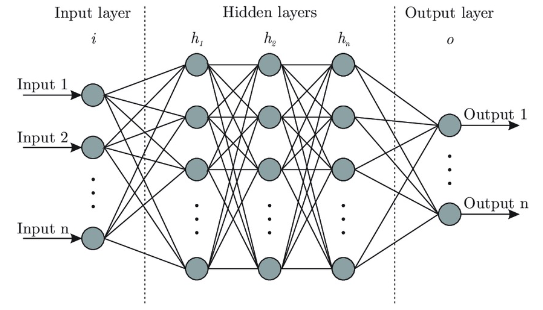
\includegraphics[width=0.68\textwidth]{Lec9/Neural networks}
%     \caption{Neural networks}
% \end{figure}

\begin{figure}[H]
    \centering
    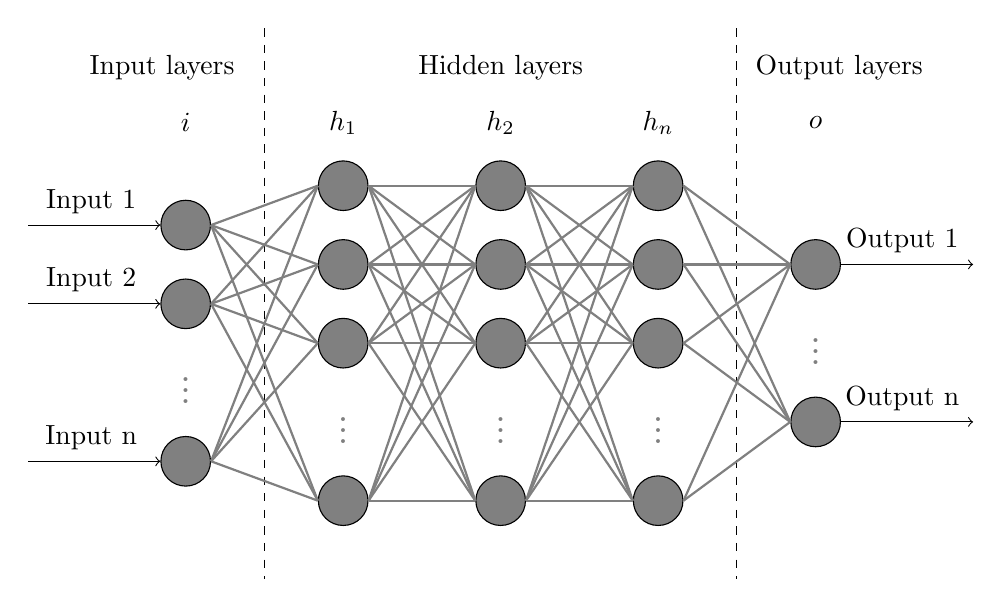
\begin{tikzpicture}
        \node (h11)    at (-2, 2) [circle, draw=black, fill=gray, text width=1em] {};
        \node (h12)    at (-2, 1) [circle, draw=black, fill=gray, text width=1em] {};
        \node (h13)    at (-2, 0) [circle, draw=black, fill=gray, text width=1em] {};
        \node (h1vdot) at (-2,-1) {\LARGE\color{gray}{$\vdots$}};
        \node (h14)    at (-2,-2) [circle, draw=black, fill=gray, text width=1em] {};

        \node (h21)    at (0, 2) [circle, draw=black, fill=gray, text width=1em] {};
        \node (h22)    at (0, 1) [circle, draw=black, fill=gray, text width=1em] {};
        \node (h23)    at (0, 0) [circle, draw=black, fill=gray, text width=1em] {};
        \node (h2vdot) at (0,-1) {\LARGE\color{gray}{$\vdots$}};
        \node (h24)    at (0,-2) [circle, draw=black, fill=gray, text width=1em] {};

        \node (h31)    at (2, 2) [circle, draw=black, fill=gray, text width=1em] {};
        \node (h32)    at (2, 1) [circle, draw=black, fill=gray, text width=1em] {};
        \node (h33)    at (2, 0) [circle, draw=black, fill=gray, text width=1em] {};
        \node (h3vdot) at (2,-1) {\LARGE\color{gray}{$\vdots$}};
        \node (h34)    at (2,-2) [circle, draw=black, fill=gray, text width=1em] {};

        \node (i1)    at (-4, 1.5) [circle, draw=black, fill=gray, text width=1em] {};
        \node (i2)    at (-4, 0.5) [circle, draw=black, fill=gray, text width=1em] {};
        \node (ivdot) at (-4,-0.5) {\LARGE\color{gray}{$\vdots$}};
        \node (i3)    at (-4,-1.5) [circle, draw=black, fill=gray, text width=1em] {};

        \draw [color=black,->] (-6, 1.5)--(i1);
        \draw [color=black,->] (-6, 0.5)--(i2);
        \draw [color=black,->] (-6,-1.5)--(i3);
        
        \node at (-5.2, 1.8) {Input 1};
        \node at (-5.2, 0.8) {Input 2};
        \node at (-5.2,-1.2) {Input n};

        \node (o1)    at ( 4, 1) [circle, draw=black, fill=gray, text width=1em] {};
        \node (ovdot) at ( 4, 0) {\LARGE\color{gray}{$\vdots$}};
        \node (o2)    at ( 4,-1) [circle, draw=black, fill=gray, text width=1em] {};

        \draw [color=black,->] (o1)--(6, 1);
        \draw [color=black,->] (o2)--(6,-1);

        \node at (5.1, 1.3) {Output 1};
        \node at (5.1,-0.7) {Output n};

        \node at (-4,2.8) {$i$};
        \node at ( 4,2.8) {$o$};
        \node at (-2,2.8) {$h_1$};
        \node at ( 0,2.8) {$h_2$};
        \node at ( 2,2.8) {$h_n$};

        \node at (-4.3,3.5) {Input layers};
        \node at (   0,3.5) {Hidden layers};
        \node at ( 4.3,3.5) {Output layers};

        \draw [dashed] (-3, 4)--(-3,-3);
        \draw [dashed] ( 3, 4)--( 3,-3);

        \foreach \x in {i1,i2,i3}{\foreach \y in {h11,h12,h13,h14}{\draw [thick,gray] (\x.east)--(\y.west);}}
        \foreach \x in {h11,h12,h13,h14}{\foreach \y in {h21,h22,h23,h24}{\draw [thick,gray] (\x.east)--(\y.west);}}
        \foreach \x in {h21,h22,h23,h24}{\foreach \y in {h31,h32,h33,h34}{\draw [thick,gray] (\x.east)--(\y.west);}}
        \foreach \x in {h31,h32,h33,h34}{\foreach \y in {o1,o2}{\draw [thick,gray] (\x.east)--(\y.west);}}
    \end{tikzpicture}
    \caption{Neural networks}
\end{figure}


输入, 隐层, 输出, 边对应着权重. 

\begin{enumerate}
    \item (Artificial) neural networks – linear functions chained together and separated by non-linear activation functions. (神经网络就是线性分类器的叠加, 用非线性激活函数分隔)
    \item Used to regress the function that maps input to output.
    \item A computational model inspired by human nervous system.
\end{enumerate}

为何叫神经网络: 与人脑应该比较接近(主要是人脑运作机制不清楚)

\begin{figure}[H]
    \centering
    \begin{minipage}{0.48\textwidth}
        \centering
        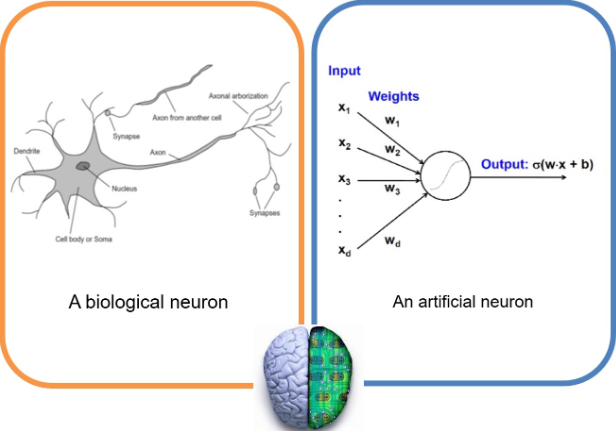
\includegraphics[width=\textwidth]{Lec9/Artificial neuron}
        \caption{Artificial neuron}
    \end{minipage}
    \begin{minipage}{0.48\textwidth}
        \centering
        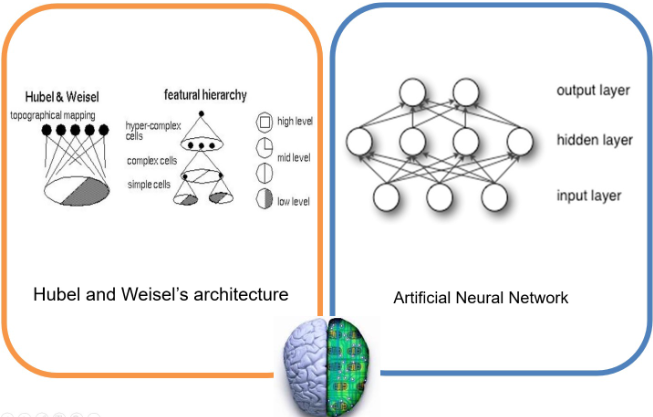
\includegraphics[width=\textwidth]{Lec9/Artificial neural networks}
        \caption{Artificial neural networks}
    \end{minipage}
\end{figure}

\subsection{Deep Neural networks}
\begin{enumerate}
    \item Deep neural networks: neural networks with many layers
    \item A network with more layers mean is able to represent more complex function
    \item The more the better?
    \begin{enumerate}
        \item More parameters to learn: need more data
        \item More difficult to train: ``gradient vanishing''
    \end{enumerate}
\end{enumerate}

\subsection{Fully connected layer(全连接层)}
所有结点与上一层链接. 
\begin{align*}
    f(x)=\sigma(Wx+b)
\end{align*}

\section{Convolutional neuarl networks}
卷积神经网络
\begin{figure}[H]
    \centering
    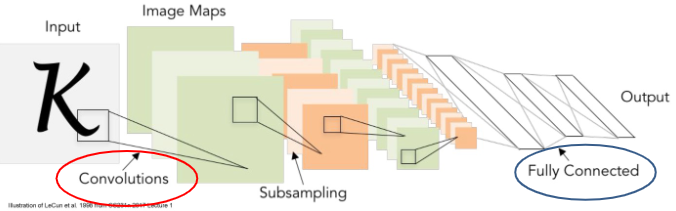
\includegraphics[width=0.68\textwidth]{Lec9/Convolutional neural networks}
    \caption{Convolutional neural networks}
\end{figure}
\subsection{Reason}

\subsubsection{Locally connected network}
全连接参数过多, 使用局部链接. 
\begin{figure}[H]
    \centering
    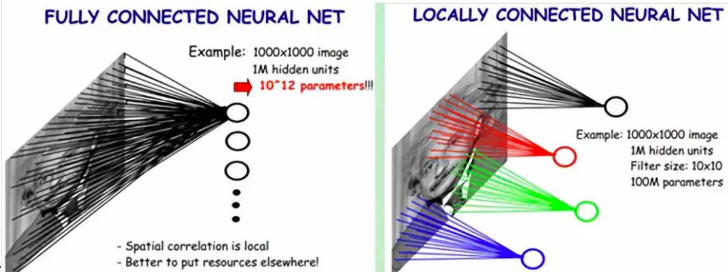
\includegraphics[width=0.68\textwidth]{Lec9/Locally connected network}
    \caption{Locally connected network}
\end{figure}

\subsubsection{Weight sharing}

局部链接参数还是太多, 使用相同的参数处理链接. 
Why is weight sharing a valid assumption?
\begin{itemize}
    \item Reminder: weights represent how an object
    should look like. (全局相似)
    \item Should not change with its position in the image(Shift invariance property,平移的不变性) 
\end{itemize}

% \begin{figure}[H]
%     \centering
%     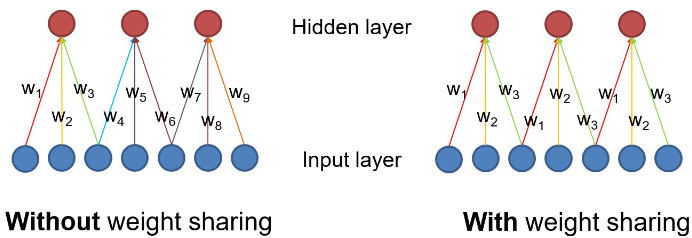
\includegraphics[width=0.74\textwidth]{Lec9/weight sharing}
%     \caption{weight sharing}
% \end{figure}

\begin{figure}[H]
    \centering
    \begin{tikzpicture}[yscale=0.8,xscale=0.8]
        \node (r1) [circle,fill=light_red,draw=black,text width=1em] at (-2,4) {};
        \node (r2) [circle,fill=light_red,draw=black,text width=1em] at ( 0,4) {};
        \node (r3) [circle,fill=light_red,draw=black,text width=1em] at ( 2,4) {};

        \node (b1) [circle,fill=light_blue,draw=black,text width=1em] at (-3,0) {};
        \node (b2) [circle,fill=light_blue,draw=black,text width=1em] at (-2,0) {};
        \node (b3) [circle,fill=light_blue,draw=black,text width=1em] at (-1,0) {};
        \node (b4) [circle,fill=light_blue,draw=black,text width=1em] at ( 0,0) {};
        \node (b5) [circle,fill=light_blue,draw=black,text width=1em] at ( 1,0) {};
        \node (b6) [circle,fill=light_blue,draw=black,text width=1em] at ( 2,0) {};
        \node (b7) [circle,fill=light_blue,draw=black,text width=1em] at ( 3,0) {};

        \draw [thick, light_red , ->]   (b1)--(r1);
        \draw [thick, yellow , ->]      (b2)--(r1);
        \draw [thick, light_green , ->] (b3)--(r1);

        \node at ( -2.8, 2) {$\mathbf{w_1}$};
        \node at ( -2, 1.2) {$\mathbf{w_2}$};
        \node at ( -1.2, 2) {$\mathbf{w_3}$};

        \draw [thick, cyan , ->]        (b3)--(r2);
        \draw [thick, black , ->]       (b4)--(r2);
        \draw [thick, brown , ->]       (b5)--(r2);

        \node at ( -0.8, 1.2) {$\mathbf{w_4}$};
        \node at ( 0, 2)      {$\mathbf{w_5}$};
        \node at ( 0.8, 1.2)  {$\mathbf{w_6}$};

        \draw [thick, gray , ->]        (b5)--(r3);
        \draw [thick, purple , ->]      (b6)--(r3);
        \draw [thick, orange , ->]      (b7)--(r3);

        \node at ( 1.2, 2) {$\mathbf{w_7}$};
        \node at ( 2, 1.2) {$\mathbf{w_8}$};
        \node at ( 2.8, 2) {$\mathbf{w_9}$};

        \node at (0,-1.2) {\textbf{Without} weight sharing};

        \node at (5,0) {Input layer};
        \node at (5,4) {Hidden layer};

        \node (r1) [circle,fill=light_red,draw=black,text width=1em] at ( 8,4) {};
        \node (r2) [circle,fill=light_red,draw=black,text width=1em] at (10,4) {};
        \node (r3) [circle,fill=light_red,draw=black,text width=1em] at (12,4) {};

        \node (b1) [circle,fill=light_blue,draw=black,text width=1em] at ( 7,0) {};
        \node (b2) [circle,fill=light_blue,draw=black,text width=1em] at ( 8,0) {};
        \node (b3) [circle,fill=light_blue,draw=black,text width=1em] at ( 9,0) {};
        \node (b4) [circle,fill=light_blue,draw=black,text width=1em] at (10,0) {};
        \node (b5) [circle,fill=light_blue,draw=black,text width=1em] at (11,0) {};
        \node (b6) [circle,fill=light_blue,draw=black,text width=1em] at (12,0) {};
        \node (b7) [circle,fill=light_blue,draw=black,text width=1em] at (13,0) {};

        \draw [thick, light_red , ->]   (b1)--(r1);
        \draw [thick, yellow , ->]      (b2)--(r1);
        \draw [thick, light_green , ->] (b3)--(r1);

        \node at ( 7.2, 2) {$\mathbf{w_1}$};
        \node at ( 8, 1.2) {$\mathbf{w_2}$};
        \node at ( 8.8, 2) {$\mathbf{w_3}$};

        \draw [thick, light_red , ->]   (b3)--(r2);
        \draw [thick, yellow , ->]      (b4)--(r2);
        \draw [thick, light_green , ->] (b5)--(r2);

        \node at (9.2, 1.2)   {$\mathbf{w_1}$};
        \node at (10, 2)      {$\mathbf{w_2}$};
        \node at (10.8, 1.2)  {$\mathbf{w_3}$};

        \draw [thick, light_red , ->]   (b5)--(r3);
        \draw [thick, yellow , ->]      (b6)--(r3);
        \draw [thick, light_green , ->] (b7)--(r3);

        \node at (11.2, 2) {$\mathbf{w_1}$};
        \node at (12, 1.2) {$\mathbf{w_2}$};
        \node at (12.8, 2) {$\mathbf{w_3}$};

        \node at (10,-1.2) {\textbf{With} weight sharing};

    \end{tikzpicture}
    \caption{weight sharing}
\end{figure}


\subsubsection{Convolution}

\begin{wrapfigure}{r}{0.38\textwidth}
    \centering
    \begin{minipage}{0.3\textwidth}
        \centering
        \begin{tikzpicture}
            \coordinate (O) at (0, 0,0);
            \coordinate (A) at (2, 0,0);
            \coordinate (B) at (2,-2,0);
            \coordinate (C) at (0,-2,0);
            \coordinate (D) at (0, 0,-0.5);
            \coordinate (E) at (2, 0,-0.5);
            \coordinate (F) at (2,-2,-0.5);
            \coordinate (G) at (0,-2,-0.5);
    
            \draw [light_blue, fill=light_blue!5] (O)--(A)--(B)--(C)--cycle;
            \draw [light_blue, fill=light_blue!5] (O)--(D)--(E)--(A)--cycle;
            \draw [light_blue, fill=light_blue!5] (A)--(B)--(F)--(E)--cycle;
    
            \draw [light_blue, fill=light_blue!60] (O)--(1.2,0,0)--(1.2,-1.2,0)--(0,-1.2,0)--cycle;
    
            \foreach \x in{1,2,...,4} \draw [light_blue] (0.4*\x,0,-0.5)--(0.4*\x,0,0)--(0.4*\x,-2,0);
            \foreach \y in{1,2,...,4} \draw [light_blue] (0,-0.4*\y,0)--(2,-0.4*\y,0)--(2,-0.4*\y,-0.5);
           
            \coordinate (O) at (  0,   0,2);
            \coordinate (A) at (0.4,   0,2);
            \coordinate (B) at (0.4,-0.4,2);
            \coordinate (C) at (  0,-0.4,2);
            \coordinate (D) at (  0,   0,2.3);
            \coordinate (E) at (0.4,   0,2.3);
            \coordinate (F) at (0.4,-0.4,2.3);
            \coordinate (G) at (  0,-0.4,2.3);
    
            \draw [black] (O)--(0,0,0);
            \draw [black] (A)--(1.2, 0,0);
            \draw [black] (B)--(1.2,-1.2,0);
            \draw [black] (C)--(0,-1.2,0);
    
            \draw [black,fill=white] (D)--(E)--(F)--(G)--cycle;
            \draw [black,fill=white] (D)--(E)--(A)--(O)--cycle;
            \draw [black,fill=white] (F)--(E)--(A)--(B)--cycle;
    
        \end{tikzpicture}
        \caption{2D convolution}
    \end{minipage}
\end{wrapfigure}

Local connectivity + weight sharing = convolution
\begin{figure}[H]
    \centering
    \begin{tikzpicture}[yscale=0.4,xscale=0.4]
        \node (r1) [circle,fill=light_red,draw=black,] at (-2,4) {};
        \node (r2) [circle,fill=light_red,draw=black,] at ( 0,4) {};
        \node (r3) [circle,fill=light_red,draw=black,] at ( 2,4) {};

        \node (b1) [circle,fill=light_blue,draw=black,] at (-3,0) {};
        \node (b2) [circle,fill=light_blue,draw=black,] at (-2,0) {};
        \node (b3) [circle,fill=light_blue,draw=black,] at (-1,0) {};
        \node (b4) [circle,fill=light_blue,draw=black,] at ( 0,0) {};
        \node (b5) [circle,fill=light_blue,draw=black,] at ( 1,0) {};
        \node (b6) [circle,fill=light_blue,draw=black,] at ( 2,0) {};
        \node (b7) [circle,fill=light_blue,draw=black,] at ( 3,0) {};

        \draw [thick, light_red , ->]   (b1)--(r1);
        \draw [thick, yellow , ->]      (b2)--(r1);
        \draw [thick, light_green , ->] (b3)--(r1);

        \node at ( -2.8, 2) {$\mathbf{w_1}$};
        \node at ( -2, 1.2) {$\mathbf{w_2}$};
        \node at ( -1.2, 2) {$\mathbf{w_3}$};

        \draw [thick, light_red , ->]   (b3)--(r2);
        \draw [thick, yellow , ->]      (b4)--(r2);
        \draw [thick, light_green , ->] (b5)--(r2);

        \node at ( -0.8, 1.2) {$\mathbf{w_1}$};
        \node at ( 0, 2)      {$\mathbf{w_2}$};
        \node at ( 0.8, 1.2)  {$\mathbf{w_3}$};

        \draw [thick, light_red , ->]   (b5)--(r3);
        \draw [thick, yellow , ->]      (b6)--(r3);
        \draw [thick, light_green , ->] (b7)--(r3);

        \node at ( 1.2, 2) {$\mathbf{w_1}$};
        \node at ( 2, 1.2) {$\mathbf{w_2}$};
        \node at ( 2.8, 2) {$\mathbf{w_3}$};
    \end{tikzpicture}
    % 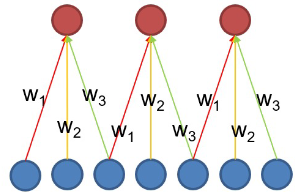
\includegraphics[width=\textwidth]{Lec9/Convolution}
    \caption{Convolution}
\end{figure}


\begin{align*}
    y=\sigma(x\otimes w +b)
\end{align*}

\subsection{Convolution}
\subsubsection{2D convolution}

The size of output is $ImageSize-FilterSize+1$. 

\subsubsection{Padding and stride}
% \begin{figure}[H]
%     \centering
%     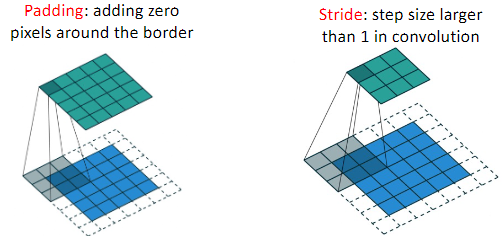
\includegraphics[width=0.68\textwidth]{Lec9/Padding and stride}
%     \caption{Padding and stride}
% \end{figure}

\begin{figure}[H]
    \centering
    \begin{minipage}{0.48\textwidth}
        \centering
        \begin{tikzpicture}
            \coordinate (A) at (0  ,0,  0);
            \coordinate (B) at (2.8,0,  0);
            \coordinate (C) at (2.8,0,2.8);
            \coordinate (D) at (0,  0,2.8);
    
            \draw [dashed,black] (A)--(B)--(C)--(D)--cycle;
            \foreach \x in {1,...,6} \draw [dashed,black] (0.4*\x,0,0)--(0.4*\x,0,2.8);
            \foreach \x in {1,...,6} \draw [dashed,black] (0,0,0.4*\x)--(2.8,0,0.4*\x);
    
            \coordinate (A) at (0.4,0,0.4);
            \coordinate (B) at (2.4,0,0.4);
            \coordinate (C) at (2.4,0,2.4);
            \coordinate (D) at (0.4,0,2.4);
    
            \draw [black,fill=light_blue] (A)--(B)--(C)--(D)--cycle;
            \foreach \x in {2,...,5} \draw [black] (0.4*\x,0,0.4)--(0.4*\x,0,2.4);
            \foreach \x in {2,...,5} \draw [black] (0.4,0,0.4*\x)--(2.4,0,0.4*\x);
    
            \coordinate (A) at (1.6,0,1.6);
            \coordinate (B) at (2.8,0,1.6);
            \coordinate (C) at (2.8,0,2.8);
            \coordinate (D) at (1.6,0,2.8);
    
            \draw [black,fill=black,opacity=0.6] (A)--(B)--(C)--(D)--cycle;
            \foreach \x in {2,2.4} \draw [black,opacity=0.6] (1.6,0,\x)--(2.8,0, \x);
            \foreach \x in {2,2.4} \draw [black,opacity=0.6] ( \x,0,1.6)--( \x,0,2.8);
    
            \draw [black!60] (A)--(  2,2,  2);
            \draw [black!60] (B)--(2.4,2,  2);
            \draw [black!60] (C)--(2.4,2,2.4);
            \draw [black!60] (D)--(  2,2,2.4);
    
            \coordinate (A) at (0.4,2,0.4);
            \coordinate (B) at (2.4,2,0.4);
            \coordinate (C) at (2.4,2,2.4);
            \coordinate (D) at (0.4,2,2.4);
    
            \draw [black,fill=light_green] (A)--(B)--(C)--(D)--cycle;
            \foreach \x in {2,...,5} \draw [black] (0.4*\x,2,0.4)--(0.4*\x,2,2.4);
            \foreach \x in {2,...,5} \draw [black] (0.4,2,0.4*\x)--(2.4,2,0.4*\x);
    
            \coordinate (A) at (  2,2,  2);
            \coordinate (B) at (2.4,2,  2);
            \coordinate (C) at (2.4,2,2.4);
            \coordinate (D) at (  2,2,2.4);
    
            \draw [black,fill=black,opacity=0.6] (A)--(B)--(C)--(D)--cycle;
        \end{tikzpicture}
        \caption{\textbf{Padding}: adding zero pixels around the border}
    \end{minipage}
    \begin{minipage}{0.48\textwidth}
        \centering
        \begin{tikzpicture}
            \coordinate (A) at (0  ,0,  0);
            \coordinate (B) at (2.8,0,  0);
            \coordinate (C) at (2.8,0,2.8);
            \coordinate (D) at (0,  0,2.8);
    
            \draw [dashed,black] (A)--(B)--(C)--(D)--cycle;
            \foreach \x in {1,...,6} \draw [dashed,black] (0.4*\x,0,0)--(0.4*\x,0,2.8);
            \foreach \x in {1,...,6} \draw [dashed,black] (0,0,0.4*\x)--(2.8,0,0.4*\x);
    
            \coordinate (A) at (0.4,0,0.4);
            \coordinate (B) at (2.4,0,0.4);
            \coordinate (C) at (2.4,0,2.4);
            \coordinate (D) at (0.4,0,2.4);
    
            \draw [black,fill=light_blue] (A)--(B)--(C)--(D)--cycle;
            \foreach \x in {2,...,5} \draw [black] (0.4*\x,0,0.4)--(0.4*\x,0,2.4);
            \foreach \x in {2,...,5} \draw [black] (0.4,0,0.4*\x)--(2.4,0,0.4*\x);
    
            \coordinate (A) at (1.6,0,1.6);
            \coordinate (B) at (2.8,0,1.6);
            \coordinate (C) at (2.8,0,2.8);
            \coordinate (D) at (1.6,0,2.8);
    
            \draw [black,fill=black,opacity=0.6] (A)--(B)--(C)--(D)--cycle;
            \foreach \x in {2,2.4} \draw [black,opacity=0.6] (1.6,0,\x)--(2.8,0, \x);
            \foreach \x in {2,2.4} \draw [black,opacity=0.6] ( \x,0,1.6)--( \x,0,2.8);
    
            \draw [black!60] (A)--(  2,2,  2);
            \draw [black!60] (B)--(2.4,2,  2);
            \draw [black!60] (C)--(2.4,2,2.4);
            \draw [black!60] (D)--(  2,2,2.4);
    
            \coordinate (A) at (1.2,2,1.2);
            \coordinate (B) at (2.4,2,1.2);
            \coordinate (C) at (2.4,2,2.4);
            \coordinate (D) at (1.2,2,2.4);
    
            \draw [black,fill=light_green] (A)--(B)--(C)--(D)--cycle;
            \foreach \x in {4,5} \draw [black] (0.4*\x,2,1.2)--(0.4*\x,2,2.4);
            \foreach \x in {4,5} \draw [black] (1.2,2,0.4*\x)--(2.4,2,0.4*\x);
    
            \coordinate (A) at (  2,2,  2);
            \coordinate (B) at (2.4,2,  2);
            \coordinate (C) at (2.4,2,2.4);
            \coordinate (D) at (  2,2,2.4);
    
            \draw [black,fill=black,opacity=0.6] (A)--(B)--(C)--(D)--cycle;
        \end{tikzpicture}
        \caption{\textbf{Stride}: step size large than 1 in convolution}
    \end{minipage}
\end{figure}


\begin{figure}[H]
    \centering
    
\end{figure}


The size of output is $\frac{ImageSize-FilterSize+Padding*2}{Stride}+1$

\subsubsection{Convolution of multi-channel image(3D tensor)
}
\begin{figure}[H]
    \centering
    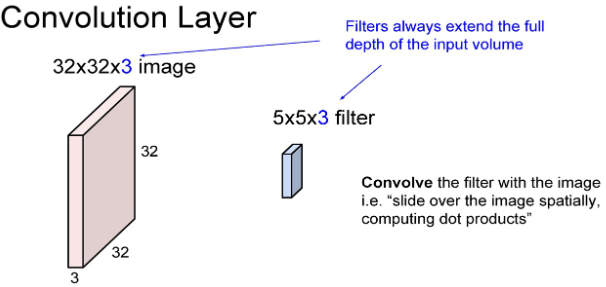
\includegraphics[width=0.48\textwidth]{Lec9/3D Convolution}
    \caption{3D Convolution}
\end{figure}

The Number of weight is $5\times 5 \times 3+1=76$ (is 3072 for fully-connected layer)

\subsection{Convolution layer}
\begin{itemize}
    \item Input: image
    \item Output: feature map (activation map)(特征图/响应图)
    \item Parameters: filter
\end{itemize}

Could be more than 1 filter. The output are multiple feature maps. Number of filters = number of feature maps

\begin{figure}[H]
    \centering
    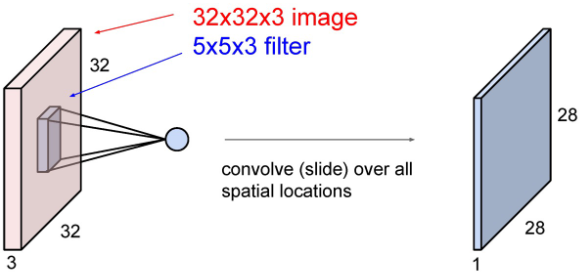
\includegraphics[width=0.48\textwidth]{Lec9/Convolution layer}
    \caption{Convolution layer}
\end{figure}

\subsection{Convolution neural network(CNN)}
CNN is a sequence of convolution layers separated by activation functions. 

\begin{figure}[H]
    \centering
    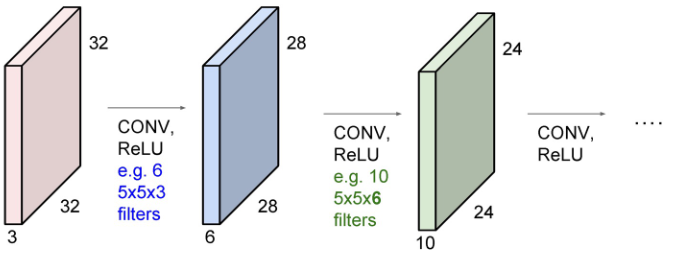
\includegraphics[width=0.48\textwidth]{Lec9/Convolution neural network}
    \caption{Convolution neural network}
\end{figure}

\begin{wrapfigure}{r}{0.38\textwidth}
    \centering
    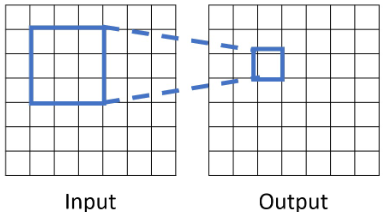
\includegraphics[width=0.28\textwidth]{Lec9/Receptive fields}
    \caption{Receptive fields}
\end{wrapfigure}

Reminder: neural network is a sequence of linear functions seperated by activation functions. 

\subsubsection{Receptive fields((可视域))}


A convolution layer with kernel size K, each element in the output depends on K x K receptive field in the input. 

For successive convolution with K kernel size and L layers, the receptive field is 1 + L * (K – 1). 

\begin{figure}[H]
    \centering
    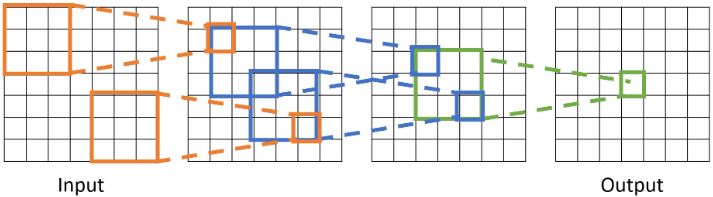
\includegraphics[width=0.48\textwidth]{Lec9/successive convolution}
    \caption{successive convolution}
\end{figure}

\subsubsection{Pooling(池化) layer}

Pooling: combine outputs of a filter at different locations. 

\begin{wrapfigure}[5]{r}{0.38\textwidth}
	\centering
    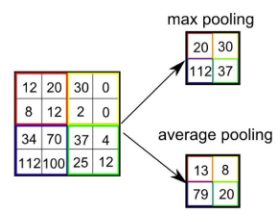
\includegraphics[width=0.18\textwidth]{Lec9/Pooling operators}
    \caption{Pooling operators}
\end{wrapfigure}

Pooling operators: 
\begin{itemize}
    \item Max pooling
    \item Average pooling
\end{itemize}

Pooling is to Aggregate spatial information and Makes feature maps smaller and more manageable. (整合信息并缩小特征图)

\begin{figure}[H]
    \centering
    \begin{subfigure}{0.15\textwidth}
        \centering
        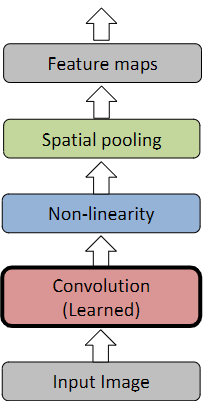
\includegraphics[width=\textwidth]{Lec9/CNN}
        \caption{CNN}
    \end{subfigure}
    \begin{subfigure}{0.48\textwidth}
        \centering
        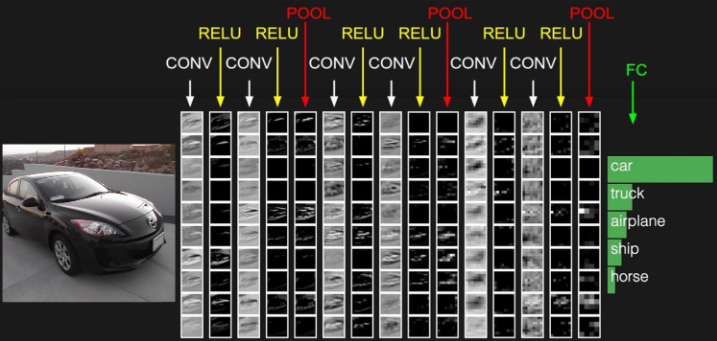
\includegraphics[width=\textwidth]{Lec9/CNN for classification}
        \caption{CNN for classification}
    \end{subfigure}
\end{figure}

结构设计比较玄学, 总的来说是利用图像特性让参数变小. 

卷积核可视化, 层级越高核越像特征的样貌. 

\section{Training neural networks}
Training: find network weights $w$ to minimize the error
between true training labels $y_i$ and estimated labels $f_w(x_i)$
\begin{align*}
    L(w)=\frac{1}{n}\sum_i l(y_i, f_w(x_i))
\end{align*}

For Example:
\begin{itemize}
    \item L2 loss for regression
    \item Cross-entropy loss for classification
\end{itemize}

Minimization can be done by gradient descent(梯度下降) provided $f$ is differentiable(可微).This training method is called back-propagation(反向传播). 

\subsection{Gradient descent}
A CNN as composition of functions
\begin{align*}
    f_w(x)=f_L(\dots(f_2(f_1(x;w_1);w_2))\dots ; w_L)
\end{align*}

Parameters

\begin{align*}
    w=(w_1,w_2,w_L)
\end{align*}

Loss function

\begin{align*}
    L(w)=\frac{1}{n}\sum_i l(y_i, f_w(x_i))
\end{align*}

Gradient descent
\begin{align*}
    w^{t+1}=w^t-\eta_t\frac{\partial L}{\partial w}(w^t)
\end{align*}
\begin{align*}
    w^{t+1}&\,\text{: New weight}\\
    w^t&\,\text{: Old weight}\\
    \eta_t&\,\text{: Learning rate}\\
    \frac{\partial L}{\partial w}(w^t)&\,\text{: Gradient}
\end{align*}

\subsection{Backpropagation}
Use chain rule to calculate gradients of loss $L$ w.r.t. weights $w$.
\begin{figure}[H]
    \centering
    \begin{tikzpicture}
        \node (z) at (0,0) [circle, draw=black,fill=light_blue] {z};
        \node (L) at (1,0) {L};

        \draw [very thick,light_green] (z)--(L);

        \node (m1) at (-2, 1.5) [circle, draw=black,fill=light_blue,text width=0.8em] {};
        \node (m2) at (-2, 0.5) [circle, draw=black,fill=light_blue] {x};
        \node (m3) at (-2,-0.5) {\LARGE$\vdots$};
        \node (m4) at (-2,-1.5) [circle, draw=black,fill=light_blue,text width=0.8em] {};

        \node (n1) at (-4, 1.7) [circle, draw=black,fill=light_blue,text width=0.8em] {};
        \node (n2) at (-4, 0.9) [circle, draw=black,fill=light_blue,text width=0.8em] {};
        \node (n3) at (-4, 0.1) {\LARGE$\vdots$};
        \node (n4) at (-4,-0.7) [circle, draw=black,fill=light_blue,text width=0.8em] {};

        \foreach \x in {m1,m2,m4} \draw [very thick,light_green] (\x.east)--(z.west);
        \foreach \x in {n1,n2,n4} \draw [very thick,light_green] (\x.east)--(m2.west);

        \foreach \x in {1.2,1.5,1.8}\draw [very thick,light_green] (m1.west)--(-2.6,\x);

        \foreach \x in {-1.2,-1.5,-1.8}\draw [very thick,light_green] (m4.west)--(-2.6,\x);

        \node at (-1,  1) {$w_1$};
        \node at (-1,0.3) {$w_2$};
        \node at (-1, -1) {$w_n$};

        \node at (-3, 1.3) {$w'_1$};
        \node at (-3, 0.7) {$w'_2$};
        \node at (-3,-0.2) {$w'_n$};

    \end{tikzpicture}
    \caption{Backpropagation}
\end{figure}

\begin{align*}
    \frac{\partial L}{\partial w_i}&=\frac{\partial z}{\partial w_i}\frac{\partial L}{\partial z}\\
    \frac{\partial L}{\partial w'_i}&=\frac{\partial x}{\partial w'_i}\frac{\partial z}{\partial x}\frac{\partial L}{\partial z}\\
\end{align*}

Algorithm:
\begin{enumerate}
    \item Forward data through the network, get loss. 
    \item Backprop to calculate the gradients. 
    \item Update the parameters using the gradient. 
    \item Go to step 1 if not converged. 
\end{enumerate}

\begin{figure}[H]
    \centering
    \begin{subfigure}{0.48\textwidth}
        \centering
        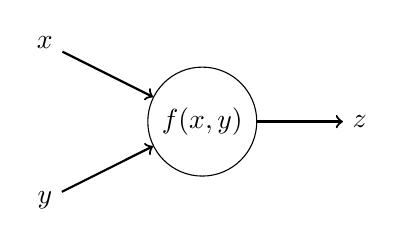
\begin{tikzpicture}
            \node (f) at (0,0) [circle,draw=black] {$f(x,y)$};
            \node (x) at (-2, 1) {$x$};
            \node (y) at (-2,-1) {$y$};
            \node (z) at ( 2, 0) {$z$};

            \draw[thick,black,->] (x)--(f);
            \draw[thick,black,->] (y)--(f);
            \draw[thick,black,->] (f)--(z);
        \end{tikzpicture}
        \caption{Forwardpass}
    \end{subfigure}
    \begin{subfigure}{0.48\textwidth}
        \centering
        \begin{tikzpicture}
            \node (f) at (0,0) [circle,light_red,draw=light_red] {$\mathrm{d}f$};
            \node (x) [color=light_red] at (-2, 1) {$\frac{\mathrm{d}L}{\mathrm{d}x}=\frac{\mathrm{d}L}{\mathrm{d}z}\frac{\mathrm{d}z}{\mathrm{d}x}$};
            \node (y) [color=light_red] at (-2,-1) {$\frac{\mathrm{d}L}{\mathrm{d}y}=\frac{\mathrm{d}L}{\mathrm{d}z}\frac{\mathrm{d}z}{\mathrm{d}y}$};
            \node (z) [color=light_red] at ( 2, 0) {$\frac{\mathrm{d}L}{\mathrm{d}z}$};

            \draw[thick,light_red,<-] (x)--(f);
            \draw[thick,light_red,<-] (y)--(f);
            \draw[thick,light_red,<-] (f)--(z);
        \end{tikzpicture}
        \caption{Backwardpass}
    \end{subfigure}
\end{figure}

\subsection{Stochastic gradient descent(SGD)}
Sometimes the training data is too large, e.g. millions of images in ImageNet. Calculate loss and gradients over all images in each iteration is too expensive. 

Stochastic gradient descent(随机梯度下降): only calcualte loss and gradients on a batch of randomly sampled images.Stochastic gradients approximate the real gradients.
\begin{align*}
    \hat{L}(w)=\frac{1}{n}\sum_{i\in \Omega}l(y_i,f_w(x_i)),\, SG=\frac{\partial \hat{L}}{\partial w}(w^t)
\end{align*}

\subsection{Architecture and hyper-parameters}

\subsubsection{Hyper-parameters(超参数)}
The number of layers to use, the number of filters in each layers, the better batch size and learning rate. 

To set them, there is one option: try them all and see what works best. (逝)

\subsubsection{Data split}
\begin{enumerate}
    \item Choose hyper-parameters that work best on the data \textcolor{light_red}{Bad: Can always decrease training loss by using a larger netwrok.} (过拟合数据)
    
    \begin{figure}[H]
        \centering
        \begin{tikzpicture}
            \node [rectangle, draw=black,fill=light_green,text width=0.68\textwidth,text centered] {Your Dataset};
        \end{tikzpicture}
    \end{figure}
    
    \item Split data into \textbf{train} and \textbf{test}, choose hyper-parameters thatwork best on test data. \textcolor{light_red}{Bad: no idea how it will perform on new data. }(过拟合test)
    
    \begin{figure}[H]
        \centering
        \begin{tikzpicture}
            \node (mid) [rectangle, draw=black,fill=light_green,text width=0.56\textwidth,text centered] {train};
            \node [rectangle, draw=black,fill=light_red,text width=0.12\textwidth,text centered] [right=0em of mid] {test};
        \end{tikzpicture}
    \end{figure}
    
    \item Split data into \textbf{train}, \textbf{validation}(验证集) and \textbf{test}, choose hpyer-parameters on validation and evaluate on test. \textcolor{light_green}{Great! Called \textbf{cross validation}(交叉验证)}
    
    \begin{figure}[H]
        \centering
        \begin{tikzpicture}
            \node (mid) [rectangle, draw=black,fill=light_green,text width=0.44\textwidth,text centered] {train};
            \node (val) [rectangle, draw=black,fill=yellow,text width=0.12\textwidth,text centered] [right=0em of mid] {validation};
            \node [rectangle, draw=black,fill=light_red,text width=0.12\textwidth,text centered] [right=0em of val] {test};
        \end{tikzpicture}
    \end{figure}
\end{enumerate}

\begin{figure}[H]
    \centering
    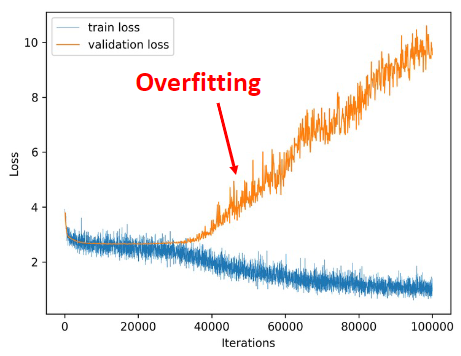
\includegraphics[width=0.38\textwidth]{Lec9/Data split}
    \caption{Overfit on train}
\end{figure}

loss的波动是因为梯度选择是随机的(SGD). 可以提前停止防止overfit. 

\subsubsection{To pick hyper-parameters}
\begin{enumerate}
    \item Train for original model.
    \item Validate to find hyper-parameters.
    \item Test to understand generalizability.
\end{enumerate}

\subsection{Overfitting}
Overfit原因之一是网络过于复杂, 使用正则来使一些参数无效化. 或者数据量过少, 有噪声, 或有 corner case. 

\subsubsection{Regularization}
\begin{align*}
    L=\frac{1}{N}\sum_{i=1}^N \sum_{j\ne y_i} \max\left( 0,f\left(x_i;W\right)_j-f\left(x_i;W\right)_{y_i}+1 \right)+\fcolorbox{light_red}{white}{$\lambda R(W)$}
\end{align*}

In commom use: 
\begin{itemize}
    \item L2: $R(W)=\sum_k \sum_l W_{k,l}^2$
    \item L1: $R(W)=\sum_k \sum_l \left|W_{k,l}\right|$
\end{itemize}

\subsubsection{Dropout}
Dropout可以证明与L2 Regularization 作用相似. 

\begin{figure}[H]
    \centering
    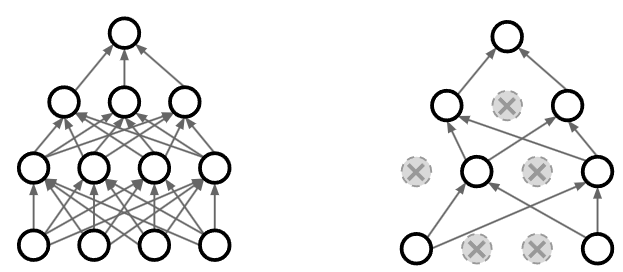
\includegraphics[width=0.68\textwidth]{Lec9/Dropout}
    \caption{Dropout}
\end{figure}

\subsubsection{Data augmentation(数据增广)}
人为创造数据

\begin{figure}[H]
    \centering
    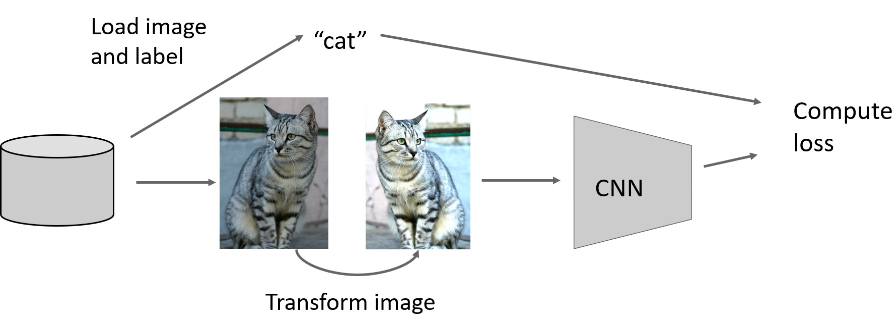
\includegraphics[width=0.68\textwidth]{Lec9/Data augmentation}
    \caption{Data augmentation}
\end{figure}

改变亮度, 模糊, 几何变换, 裁剪图像等. 

\subsubsection{To prevent overfitting}
\begin{itemize}
    \item Cross validation and early stop.
    \item Regularization or dropout.
    \item Data augmentation. 
\end{itemize}

\subsection{Batch Normalization(归一化)}
Normalize the outputs of a layer so they have zero mean and unit variance. To reduce internal covariate shift.
\begin{align*}
    \hat{x}^{(k)}=\frac{x^{(k)}-\mathrm{E}\left[x^{(k)}\right]}{\sqrt{\mathrm{Var}\left[x^{(k)}\right]}}
\end{align*}

Input: $x \in N \times D$, $N$ is channels, $D$ is $B*H*W$ for a batch of images.

\begin{multicols}{2}
    \begin{align*}
        \mu_j&=\frac{1}{N}\sum_{i=1}^N x_{i,j}\\
        \sigma_j^2&=\frac{1}{N}\sum_{i=1}^{N}(x_{i,j}-\mu_j)^2\\
        \hat{x}_{i,j}&=\frac{x_{i,j}-\mu_j}{\sqrt{\sigma_j^2+\varepsilon }}
    \end{align*}
    \columnbreak
    \begin{figure}[H]
        \centering
        \begin{tikzpicture}
            \node (m) [rectangle,draw=black,fill=gray,text width=8em,text centered, minimum height=8em] {X};
            \node [ left=1em of m] {N};
            \node [below=1em of m] {D};
        \end{tikzpicture}
    \end{figure}
\end{multicols}

Usually inserted after FC / Conv and before nonlinearity.

Advantages:
\begin{itemize}
    \item Much easier to train.
    \item Allow higher learning rate, faster convergence.
    \item More robust to initialization. 
\end{itemize}

\subsection{Deep learning frameworks}
Support fast development of deep learning algorithms.

Various modules to build a network: operations, layers, losses. 

Various optimizers to train networks with CPU/GPU/Multiple GPUs.

\begin{itemize}
    \item Caffe 早
    \item TensorFlow 便于部署, 工程化
    \item PyTorch 上手容易, 研究使用多
\end{itemize}

\section{Network architectures}
历史
\begin{enumerate}
    \item 以前数据集小, 有过拟合, 且网络难以训练. 
    \item ImageNet: 巨大的图像数据集. 
    \item GPU: 矩阵并行, NVIDIA的cuda. 
    \item AlexNet: 在ImageNet展示了深度学习的强大, 其在图像分类上减到了16\%, 甚至到7\%
    \begin{figure}[H]
        \centering
        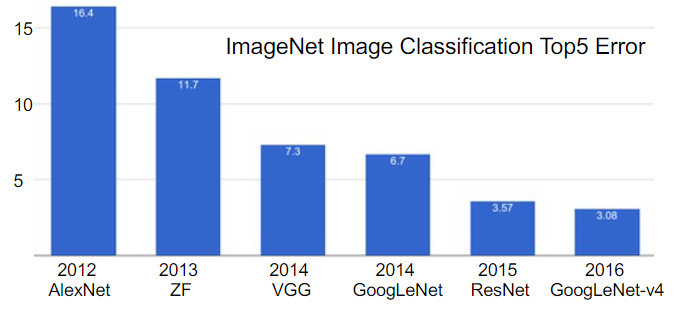
\includegraphics[width=0.38\textwidth]{Lec9/Progress on ImageNet}
        \caption{Progress on ImageNet}
    \end{figure}
    
    现在 ResNet 用的多. 
    \item ResNet: 增加层数但loss变大. 
    
    设计一种网络, 使加一层但loss不会变大, 尝试训练出一种空白层(identity map)过于困难, 于是构造并训练一种空白层, 相当于用网络去学习输入到输出的残差, 而不是直接输入到输出, 如此就叫残差网络. 即使用残差逼近原来的输出. 
    
    \begin{figure}[H]
        \centering
        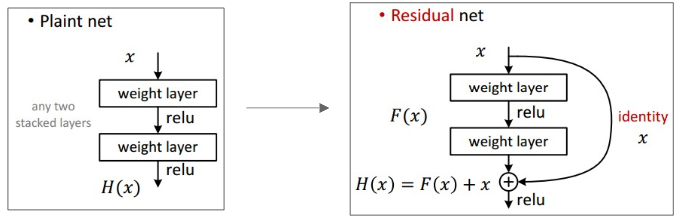
\includegraphics[width=0.38\textwidth]{Lec9/ResNet}
        \caption{ResNet}
    \end{figure}
    
    梯度消失: 层数过多时梯度会越来越小以至于消失. 

    残差网络减弱了梯度消失. 

    \item DenseNet: 每层输入会连到前面的输出, 相当于更多的残差. 
    \begin{figure}[H]
        \centering
        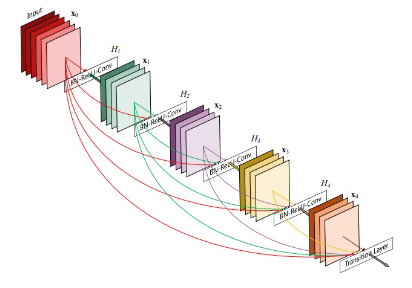
\includegraphics[width=0.38\textwidth]{Lec9/DenseNet}
        \caption{DenseNet}
    \end{figure}
    
    \item MobileNets: 快! 可在移动端上运行. 
    \item Neural architecture search: 自己调自己, 自己试自己. (套娃)
\end{enumerate}
